\documentclass{sigchi}

% Use this command to override the default ACM copyright statement (e.g. for preprints). 
% Consult the conference website for the camera-ready copyright statement.


%% EXAMPLE BEGIN -- HOW TO OVERRIDE THE DEFAULT COPYRIGHT STRIP -- (July 22, 2013 - Paul Baumann)
% \toappear{Permission to make digital or hard copies of all or part of this work for personal or classroom use is 	granted without fee provided that copies are not made or distributed for profit or commercial advantage and that copies bear this notice and the full citation on the first page. Copyrights for components of this work owned by others than ACM must be honored. Abstracting with credit is permitted. To copy otherwise, or republish, to post on servers or to redistribute to lists, requires prior specific permission and/or a fee. Request permissions from permissions@acm.org. \\
% {\emph{CHI'14}}, April 26--May 1, 2014, Toronto, Canada. \\
% Copyright \copyright~2014 ACM ISBN/14/04...\$15.00. \\
% DOI string from ACM form confirmation}
%% EXAMPLE END -- HOW TO OVERRIDE THE DEFAULT COPYRIGHT STRIP -- (July 22, 2013 - Paul Baumann)


% Arabic page numbers for submission. 
% Remove this line to eliminate page numbers for the camera ready copy
% \pagenumbering{arabic}


% Load basic packages
\usepackage{balance}  % to better equalize the last page
\usepackage{graphics} % for EPS, load graphicx instead
\usepackage{times}    % comment if you want LaTeX's default font
\usepackage{url}      % llt: nicely formatted URLs

% llt: Define a global style for URLs, rather that the default one
\makeatletter
\def\url@leostyle{%
  \@ifundefined{selectfont}{\def\UrlFont{\sf}}{\def\UrlFont{\small\bf\ttfamily}}}
\makeatother
\urlstyle{leo}


% To make various LaTeX processors do the right thing with page size.
\def\pprw{8.5in}
\def\pprh{11in}
\special{papersize=\pprw,\pprh}
\setlength{\paperwidth}{\pprw}
\setlength{\paperheight}{\pprh}
\setlength{\pdfpagewidth}{\pprw}
\setlength{\pdfpageheight}{\pprh}

% Make sure hyperref comes last of your loaded packages, 
% to give it a fighting chance of not being over-written, 
% since its job is to redefine many LaTeX commands.
\usepackage[pdftex]{hyperref}
\hypersetup{
pdftitle={Reconstructing Browsing Activities from Browser History},
pdfauthor={LaTeX},
pdfkeywords={SIGCHI, proceedings, archival format},
bookmarksnumbered,
pdfstartview={FitH},
colorlinks,
citecolor=black,
filecolor=black,
linkcolor=black,
urlcolor=black,
breaklinks=true,
}

% create a shortcut to typeset table headings
\newcommand\tabhead[1]{\small\textbf{#1}}


% End of preamble. Here it comes the document.
\begin{document}

\title{Reconstructing Browsing Activities from Browser History}

\numberofauthors{3}
\author{
  \alignauthor 1st Author Name\\
    \affaddr{Affiliation}\\
    \affaddr{Address}\\
    \email{e-mail address}\\
    \affaddr{Optional phone number}
  \alignauthor 2nd Author Name\\
    \affaddr{Affiliation}\\
    \affaddr{Address}\\
    \email{e-mail address}\\
    \affaddr{Optional phone number}    
  \alignauthor 3rd Author Name\\
    \affaddr{Affiliation}\\
    \affaddr{Address}\\
    \email{e-mail address}\\
    \affaddr{Optional phone number}
}

\maketitle

\begin{abstract}
Users' browsing activities -- such as what sites they are spending time on and for how long, or what tabs they have open and which are focused at any given time -- is useful for a number of research and practical applications. Gathering such data, however, requires a longitudinal study in which users must install a monitoring toolkit. In contrast, a browser extension is able to instantly access months of browsing history. However, browsing histories do not include important information such as time spent. In this work we aim to reconstruct time spent on sites from browsing histories. We gathered 3 months of browsing histories, and 2 weeks of browsing activities from 150 users. We are able to reconstruct the URL the user is looking at with X\% accuracy, and total time spent on domains with an $R^2$ value of Y.
\end{abstract}

\keywords{
browsing histories; browsing activities; browser focus; web browsing
}

\category{H.5.m.}{Information Interfaces and Presentation (e.g. HCI)}{Miscellaneous}

\section{Introduction}

Knowing where users spend their time online, second-by-second, has numerous applications to both research and products. For example, productivity-tracking tools like RescueTime provide users with information about how much time they are spending on different site types. Browsing activity data is also essential for studying phenomenon such as self-interruptions, where users may take a break from work to spend time on other sites.

However, gathering browsing activity data is a long and intrusive process. It requires the end user to install a monitoring application -- such as a browser extension -- that continually logs where users are spending their time, and transmits it to a server. This requires extensive permissions which may make users wary of participation, on suspicions that the extension may be malware. The user must also keep the extension installed over the duration of the study (whereas we observed many Mechanical Turk users would simply uninstall the extension after they have been paid). Most problematically, a longitudinal study is required, with duration equivalent to the amount of browsing activity data we wish to collect.

Browsing histories, in contrast, can be instantly gathered by a browser extension. For a Chrome extension, it requires only a Browsing History permission which is classified as low-risk, and can be uninstalled as soon as the history has been transmitted to the server, which should help alleviate potential concerns that the software is malware. Most promisingly, users' browsing histories can store several months of browsing data, allowing us to instantly get results without a longitudinal study.

In this work we aim to reconstruct four pieces of browsing activity, using browsing histories:

\begin{enumerate}
	\item At what times is the browser being actively used?
	\item What tabs are open at any given time?
	\item What URL is the browser focused on at any given time?
	\item How much time did users spend overall on each domain?
\end{enumerate}

These tasks are non-trivial because the browsing history represents only events where a new page is visited, and not time spent within a page or switching/closing tabs. This makes naive time-estimation heuristics fail on pages where users might spend a long time without any record in the browsing history (ie, watching a Youtube video, or scrolling down a Facebook news feed).

To train and evaluate our reconstruction mechanism, we gathered browsing histories, and 2 weeks of second-by-second browsing activities, from 200 Mechanical Turk users. Our techniques outperform heuristics such as assuming a fixed time after a page visit, and are able to correctly reconstruct the URL the browser is focused on X\% of the time.

\section{Related Work}

Gathering browsing activities by logging it in a longitudinal study is a methodology that underlies a number of studies. For example, Mark et al have conducted studies that relate browsing activities to sleep debt \cite{mark2016sleep} and stress \cite{mark2014stress}, as well as using them to investigate social media usage \cite{wang2015coming} and multitasking \cite{mark2015focused}.

Eyebrowse is an application where users can voluntarily share their browsing activities \cite{eyebrowse}. They have gathered a dataset of browsing activities from their userbase. Although we considered using Eyebrowse's dataset for training and evaluating our model rather than collecting our own, at the time we checked it, there were only 14 users with at least 1000 logged visits, which was not enough data. Furthermore, as users only selectively share their browsing histories in the Eyebrowse system, it may be biased and underrepresent certain activities, whereas our own collected dataset represents the full range of activities that users engage in online.

Park et al investigate the relationship between video view durations on Youtube and its view count, number of likes per view, and sentiment in the comments \cite{youtubeduration}. They find that these factors have significant predictive power over the duration the video, and are able to predict the duration of video views with an $R^2$ value of 0.19.

\section{Dataset}

\subsection{Dataset Collection}

We first gathered a dataset of browsing activities and browser histories. We recruited 200 users from Mechanical Turk, and asked them to install our extension which collects browser histories, and browsing activity events (browser window and tab focus and switches, as well as mouse and keyboard activity such as clicks and scrolls on pages), and transmits it to our servers.

Users were compensated \$2 for installing the extension, and were given a bonus of \$1 for each week they kept the extension installed. We excluded users if they uninstalled the extension, became inactive for more than 3 days, or cleared their browsing history.

We were able to gather data from 150 users in this way (most of the 50 who dropped uninstalled the extension shortly after receiving the initial \$2 payment), which we then split into our training and test sets (data from 75 users in each).

\subsection{Summary Statistics}

In (some figure) we show summary statistics for our dataset. Users spend much time on Mechanical Turk (as we are sampling from a pool of Mechanical Turk users), but they also spend time browsing other, more broadly-used sites.

\subsection{Reference Browser Activity Data}

The reference browser activity dataset was obtained by logging open, close, switch, and change events for tabs and windows via Chrome's tab and window APIs for extensions. We also logged when the user's screen locks or the browser becomes idle (defined by Chrome as 1 minute without mouse or keyboard activity), via Chrome's idle API for extension. For each event, we logged which tabs and windows were open, the URLs they were visiting, and which tabs were focused.
% We also logged mouse and keyboard activities (so we can detect when the page is idle) by injecting a content script into the page.

We then transformed this data into spans of time, which record when the user starts and ends a period of activity on URL (where the start occurs when the URL is visited or gains tab focus, and the end occurs by either navigating to a different page, closing the tab or window, switching to a different tab, browser window, or application, or if the browser becomes idle or the screen is locked).

Note that a limitation of Chrome's definition of the browser being idle is that the user may still be looking at a page without mouse or keyboard activity for an extended duration of time -- they may be slowly reading a page, thinking about some diagram, or watching a video -- which will be recorded within this dataset as an idle period.

\subsection{History Data}

The history data was obtained via Chrome's history API for extensions. It includes the URL that was visited, the time it was visited at, as well as how the visit occurred (by clicking a link, reloading a page, navigation within a frame, etc).

While attempting to find the correspondences between our history data and our reference browsing activities, we found there existed some differences. Obviously, there are many events such as tab switches and time spent scrolling down a page that are only represented in the browsing activity data. However, there are also some activities that occur in the browsing history but not the browsing activity data. One type of such event is navigation within frames, which we corrected for by eliminating them from the history (the browsing history explicitly marks navigation within frames as such). % Another type of such event is browsing history events which are inserted via the history API (to aid in backwards navigation vi) -- which will contribute to errors in our evaluation (primarily, misclassification of the ).

\section{Reconstruction Procedure}

Since our ultimate goal is to be able to reconstruct, second-by-second, whether the user's browser is active and which page they are browsing, we broke this procedure into three subparts:

\begin{enumerate}
	\item Estimate the spans during which the browser is active (as opposed to the browser being closed, idle, or a different window being in focus)
	\item Estimate which URLs are open in non-focused tabs at any given point in time. This will give us a set of candidate tabs that users might switch to.
	\item Within spans in which we believe the browser to be active, estimate which URL is being browsed at each point in time.
\end{enumerate}

\section{When was the browser active?}

A baseline model for estimating when the browser was active, based on the browser history, is to simply guess that the browser remained active for some amount of time (for example, 30 seconds, 1 minute, or 2 minutes) after the last recorded event in the history.

We can evaluate the correctness of this approach by considering it as a binary classification problem for each second in the history. We consider a true positive to be when we correctly predict that the browser was active, a true negative is when we correctly predict that the browser was inactive, a false positive to be when we predict the browser was active when it was in fact inactive, and a false negative to be when we predict the browser was inactive when it was in fact active.

Results for the naive model are shown in (figures). As we can see, adjusting the time threshold enables us to trade off precision and recall, with a 5-minute threshold achieving the best F1 score on the test set.

We developed a more sophisticated model which approaches the problem as follows: during the span of time between an item in the browser history and the next item, is the majority of the time active or not? To make our decision, we consider the duration of the time between them, the domain of the current item, and the domain of the next item. Our approach takes advantage of the following three phenomenon:

\begin{enumerate}
	\item Browsing occurs in sessions -- within a session, it is more likely that the browser was continually active.
	\item The domain that occurs at the beginning of the span may influence the expected duration of the visit. It may be a domain that users tend to stay on for shorter/longer, or it may be a domain that tends to end sessions.
	\item The domain that occurs at the end of the span may influence the expected duration of the visit. It may be a domain that tends to start sessions.
\end{enumerate}

This thus becomes a classification problem where we wish to classify whether or not the browser is active during the majority of the span, given the span duration and the domains that are at the beginning and end of the span. Unfortunately, if we simply handle the domains as categorical features are usually handled (1-hot encoding each possibility), this will result in the number of features being the number of domains squared, which will lead to dimensionality problems. Instead, we handle this by training a decision tree for more common domain pairs, and backing off to more generic classifiers if insufficient data (less than 100 positive and negative samples) is available. Because the distribution is unbalanced (more positive samples than negative), during training we balance the weights for the classes. We use a decision tree classifier (limited to depth of 1) due to fast performance. In order of priority, we use:

\begin{enumerate}
	\item Classifier specific to both start and end domain
	\item Classifier specific to the start domain
	\item Classifier specific to the end domain
	\item Generic classifier trained on all data
\end{enumerate}

\begin{figure}[!h]
\centering
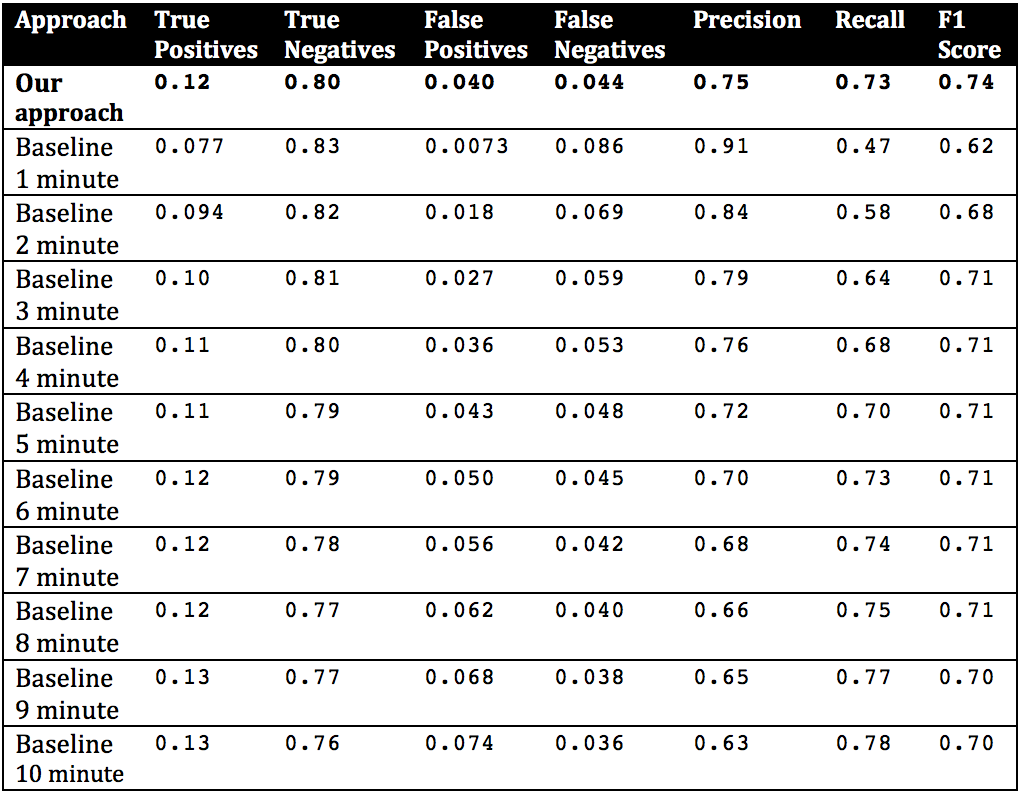
\includegraphics[width=0.9\columnwidth]{span_reconstruction_results}
\caption{Span reconstruction results. Baseline X minutes indicate the reconstruction heuristic where we assume that the browser is active up to X minutes after each history event. Our approach achieves a higher F1 score than any of the baseline approaches.}
\label{fig:spanreconstruction}
\end{figure}

The performance of this classifier on the task of predicting whether the browser is active during the majority of a span is 0.98 precision, 0.98 recall, and 0.98 F1 score. If we take these results and fill in the spans accordingly, this results in the scores shown in \autoref{fig:spanreconstruction} , where we see that our F1 score of 0.74 outperforms all of our baseline classifiers.

\section{Which tabs were open?}

Next, we determine which tabs were open at any given time. A simple heuristic to estimate this is to assume that tabs remain open for a certain number of minutes after they appear in the history. We can evaluate the correctness of our estimate by comparing, at each point in time where the set of tabs changes, to the actual tabs which are open. This is again a binary classification task: each URL that we correctly predict is open in a tab is counted as a true positive, each URL that we predict is open in a tab but is not is counted as a false positive, and each URL that is open in a tab but we did not predict is counted as a false negative.

A more sophisticated heuristic takes into account the expected lifetime of a tab, given the domain.

As shown in (figure) our results indicate that 

\section{Which URL was focused?}

Now that we have an estimation of when the browser was active, the final step is to determine which URL was focused at any given point in time.

A simple heuristic is to simply guess that for each span we reconstructed, the time of the entire span was spent at the URL at the start of the span. This heuristic works well in contexts such as single-page applications, such as an infinite-scrolling feed which the user will visit but then keep reading for several minutes. We find that on a second-by-second basis, this heuristic predicts the correct URL 69\% of the time, and predicts the correct domain 76\% of the time.

A more sophisticated heuristic takes into account the set of tabs we believe to be open. Here, for each domain that could be at the start of the span we compute a distribution of the domains we expect users will spend time on. We then pick, among the tabs we believe to be open, the URL that is most likely to have time spent on, given the starting domain.

As shown in (figure) our results indicate that 

\section{How much time was spent on each domain?}

Having now reconstructed the URLs where users spent their time on a second-by-second, we can now evaluate how accurately this can be used to compute overall time spent on domains. Overall time spent on domains is a useful piece of data that can be used in several time-tracking and productivity applications, as well as studies where time spent online or on a specific service is of interest.

We computed for each user an estimate of how much time they spent on each domain, and then computed the weighted Pearson product-moment correlation coefficient between the estimated and actual times, with each domain representing a sample weighted according to the total amount of time the user spent on it (to give more importance to the domains users spent more time on).

As shown in (figure) our results indicate that 

\section{Discussion}

Discussion will go here

\section{Conclusion}

Conclusion will go here

% Balancing columns in a ref list is a bit of a pain because you
% either use a hack like flushend or balance, or manually insert
% a column break.  http://www.tex.ac.uk/cgi-bin/texfaq2html?label=balance
% multicols doesn't work because we're already in two-column mode,
% and flushend isn't awesome, so I choose balance.  See this
% for more info: http://cs.brown.edu/system/software/latex/doc/balance.pdf
%
% Note that in a perfect world balance wants to be in the first
% column of the last page.
%
% If balance doesn't work for you, you can remove that and
% hard-code a column break into the bbl file right before you
% submit:
%
% http://stackoverflow.com/questions/2149854/how-to-manually-equalize-columns-
% in-an-ieee-paper-if-using-bibtex
%
% Or, just remove \balance and give up on balancing the last page.
%
\balance

% REFERENCES FORMAT
% References must be the same font size as other body text.

\bibliographystyle{acm-sigchi}
\bibliography{reconstruct}
\end{document}
